\documentclass[12pt, a4paper]{article}
\usepackage[utf8]{inputenc}

% Format
\usepackage{layout}
\setlength{\parindent}{0.5in}
\setcounter{secnumdepth}{0}
\usepackage{lineno}
%\usepackage{authblk}

% Font
\usepackage{MinionPro}
\input glyphtounicode
\pdfgentounicode=1
\usepackage{microtype}
\usepackage[super]{nth}

% Language
\usepackage[british]{babel}

% References
\usepackage[nosectionbib, tocbib, unnumberedbib]{apacite}

% Figures
\usepackage{graphicx}
\usepackage[small, labelfont=it, labelsep=period]{caption}

% Tables
\usepackage{booktabs}
\usepackage{tabularx}

% Commands
\newcommand{\pest}[4]{$ \text{Pr} (\text{``us''} | \text{#1}) = #2$, $[#3, #4]$}
\newcommand{\pdif}[4]{$ \Delta\text{Pr} (\text{``us''} | \text{#1}) = #2$, $[#3, #4]$}

% Frontmatter
\title{\emph{Appendices for}\\Intergroup contact fosters\\more inclusive social identities}
\date{November 5, 2018}
%\author{Nils Karl Reimer}
%\author[2]{Shanmukh V. Kamble}
%\author[3]{Katharina Schmid}
%\author[1]{Miles Hewstone}
%\affil[1]{University of Oxford}
%\affil[2]{Karnatak University}
%\affil[3]{ESEADE Business School, Ramon Llull University}
%\renewcommand\Affilfont{\small}

\begin{document}

\maketitle

\section{Appendix A: Pilot Study}

Informed by local knowledge, we intended to rely on last names to unobtrusively communicate caste membership in the crossed-categorization task. To find the most prototypical stimuli, wecompiled an initial set of 50 surnames, drawing on local knowledge, databases on naming preferences, and publicly available archives of Facebook usernames. We selected 10 surnames for each of five combinations of nationality, religion, and caste: (1) Indian Hindus of upper-caste backgrounds, (2) Indian Hindus of lower-caste backgrounds (Dalits), (3) Indian Muslims, (4) foreign Hindus, and (5) foreign Muslims. From these 50 names, we created 100 stimuli resembling identity cards, 50 with female first names and 50 with male first names. Each card had the target's first and last name, age (21--26 years), and religion (Hindu, Muslim) printed on them, as well as a flag corresponding to the target's nationality (Indian, Nepali, Sri Lankan, Bangladeshi) and a silhouette corresponding to the target's gender \cite<adapted~from>{ma_chicago_2015}. Cards for female and male targets were identical in all attributes except first name and silhouette.

We asked 26 students (19 women, 7 men) of diverse caste groups (\emph{SC/ST}: 8, \emph{GM}: 10, \emph{OBC}: 8) and religious backgrounds (\emph{Hinduism}: 16, \emph{Islam}: 4, \emph{Christianity}: 5, \emph{Jainism}: 1) to review 25 of the 50 stimuli corresponding to their gender. For each stimulus, we asked participants which caste they thought the target most likely belonged to (\emph{SC/ST}, \emph{GM}, \emph{OBC}, \emph{GM or OBC}, \emph{Can't tell/Don't know}), how typical or unusual they considered the target's name for someone of that particular nationality, religion, and (if applicable) caste $(1 = \textit{very typical}, 6 = \textit{very unusual})$, and whether the target's name reminded them of anyone in particular (\emph{yes}, \emph{no}) and, if so, of whom. 

Participants' responses had important implications for designing the crossed-categorization task. On average, participants regarded all targets' names as at least ``somewhat typical'' $(1.42 \le \textit{Ms} \le 3.50)$. Names, however, were not enough to reliably cue caste membership---only $55\%$ to $83\%$ of participants identified even the most distinctive Dalit targets as Scheduled Caste~/ Scheduled Tribe (see Figure~\ref{fig:a-1}). Further, participants consistently categorized Muslim targets as Other Backward Class (see Figure~\ref{fig:a-2}), introducing a potential confound when comparing Muslim (OBC) and Hindu (GM) targets. Considering these findings, we decided to explicitly state caste membership (as reservation categories: GM, OBC, SC/ST) for Indian targets, and to add \emph{Indian, Hindu, OBC} targets as a sixth category.

\begin{figure}
\centering
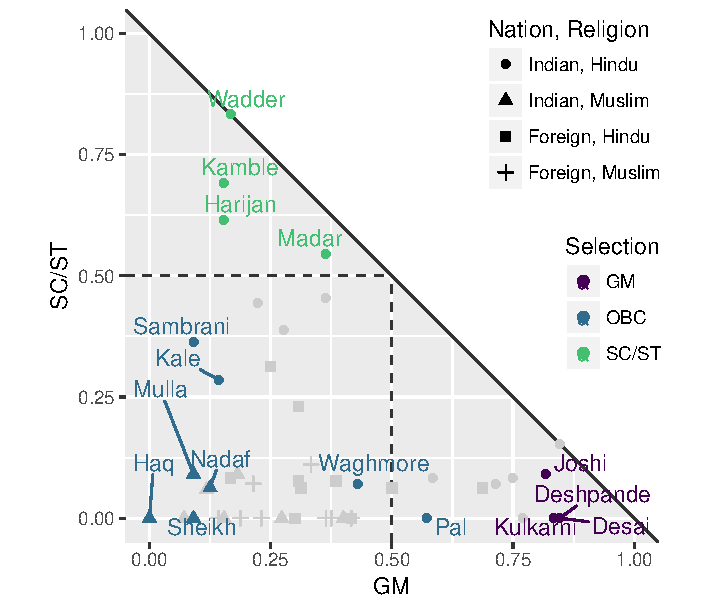
\includegraphics[scale=1]{../figures/appendices/appendices-a-1}
\caption[Proportion of SC/ST vs GM classifications per target stimulus (Pilot study)]{Proportion of SC/ST vs GM classifications per target stimulus. Targets in the upper-left quadrant were most often classified as SC/ST, while targets in the lower-right quadrant were most often classified as GM. Targets in the lower-left quadrant were more often classified as GM or OBC, or OBC than as SC/ST or GM, or could not be classified reliably. Colours highlight Indian targets selected as GM, OBC, and SC/ST stimuli, respectively, based on participants' categorizations in the pilot study. GM = General Merit, OBC = Other Backward Class, SC/ST = Scheduled Caste~/ Scheduled Tribe}
\label{fig:a-1}
\end{figure}

\begin{figure}
\centering
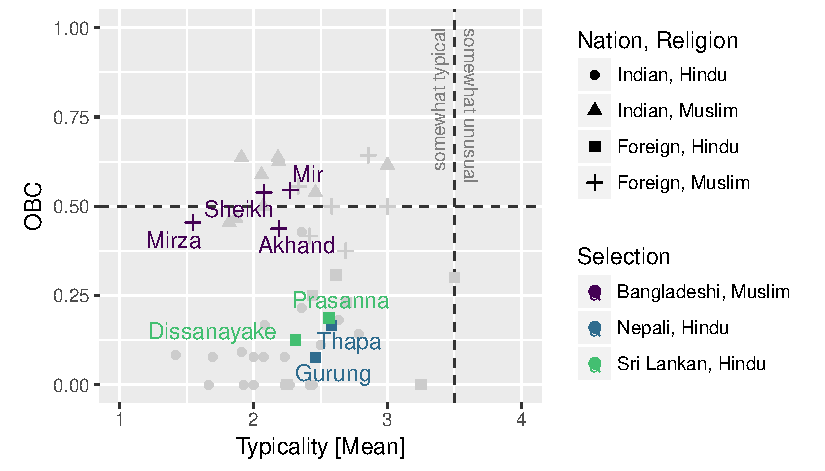
\includegraphics[scale=1]{../figures/appendices/appendices-a-2}
\caption[Foreign targets selected based on participants' average typicality ratings (Pilot study)]{Foreign targets selected as Sri Lankan, Hindu (2), Nepali, Hindu (2), and Bangladeshi, Muslim (4) stimuli, respectively, based on participants' average typicality ratings.}
\label{fig:a-2}
\end{figure}

For the final set of stimuli, we chose the four most prototypical targets for each of the six categories under study. We ranked Indian targets by the proportion of ``correct'' categorizations (e.g., $\Pr(\textit{OBC})$ for \emph{Muslim, OBC} targets) weighted by the inversed proportions of ``incorrect'' categorizations (e.g., $1 - \Pr(\textit{SCST})$ and $1 - \Pr(\textit{GM})$ for \emph{Muslim, OBC} targets). We selected the four highest-ranked (Category 1) \emph{Hindu, GM}, (2) \emph{Hindu, OBC}, (3) \emph{Hindu, SC/ST}, and (4) \emph{Muslim, OBC} targets (see Figure~\ref{fig:a-1}). We ranked foreign targets by their average typicality rating, and excluded targets who were categorized as General Merit or Scheduled Caste~/ Scheduled Tribe by $\ge 50\%$ of participants (to avoid obvious caste associations). We selected the two most typical (Category 5) \emph{Nepali, Hindu} and \emph{Sri Lankan, Hindu} targets, and the four most typical (6) \emph{Bangladeshi, Muslim} targets (see Figure~\ref{fig:a-2}). Based on the pilot study, we thus used $6~(\text{categories}) \times 4~(\text{targets}) = 24$ stimuli in the final study. Between $0\%$ and $44\%$ of participants ($\textit{Mdn} = 10\%$) recognised each selected name as familiar---in most cases, participants reported that targets reminded them of fellow students, former classmates, or co-workers.

\section{Appendix B: Social Identity Structures}

Van Dommelen et al. \citeyear{dommelen_construing_2015} analysed participants' responses as \emph{Social Identity Inclusiveness}, i.e. the total number of 24 targets a participant had categorized as ``us'', and as \emph{Social Identity Structures}, i.e. the specific structures proposed by \citeA{roccas_social_2002}. Neither measure translated well to the present study. As participants had different caste backgrounds, comparing their inclusiveness scores ($M = 15.34$, $\textit{SD} = 4.88$, $\textit{Mdn} = 16$) was less meaningful than in \citeauthor{dommelen_construing_2015}'s sample. Coding structures was interesting in principle, but proved difficult in practice.  Few (9\%, $n = 26$) participants consistently classified all targets in each category as either ``us'' or ``not us''. Relatedly, how participants classified targets within a category was correlated, but only moderately so ($.41 \leq rs \leq.66$, see Table ~\ref{tab:ch4-s4-2}). The inconsistency in participants' responses made hard and fast coding rules, as used by \citeauthor{dommelen_construing_2015}, impractical.

\begin{table}
\centering
\figureversion{lining, tabular}
\caption[Mean intra and inter-category correlations for target categorizations]{Mean \emph{intra}-category (\textbf{diagonal}) and \emph{inter}-category correlations between participants' categorizations of targets in the respective categories.}
\small	
\begin{tabular}{rlrrrr|rr} \toprule
\# & Category            & 1   & 2   & 3   & 4   & 5   & 6   \\ \midrule \addlinespace
1  & Indian, Hindu, GM   & \textbf{.48} & .56 & .33 & .43 & .16 & .08 \\
2  & Indian, Hindu, OBC  & .56 & \textbf{.41} & .29 & .46 & .09 & .06 \\
3  & Indian, Hindu, SCST & .33 & .29 & \textbf{.66} & .35 & .03 & .16 \\
4  & Indian, Muslim, OBC & .43 & .46 & .35 & \textbf{.52} & .01 & .24 \\ \midrule
5  & Foreign, Hindu      & .16 & .09 & .03 & .01 & \textbf{.50} & .47 \\
6  & Foreign, Muslim     & .08 & .06 & .16 & .24 & .47 & \textbf{.51} \\ \addlinespace \bottomrule
\end{tabular}
\label{tab:ch4-s4-2}
\end{table}

Instead, we quantified the (dis)similarity between a participant's responses and various proposed social identity structures by calculating edit distances. We operationalised \emph{edit distance} as the number of a participant's categorizations that would need to change from ``us'' to ``not us'' (and vice versa) to make them identical to the categorizations implied by a certain structure. Figure~\ref{fig:b-1} shows the distributions of participants' edit distances from each structure, as well as median edit distances. 

\begin{figure}
\centering
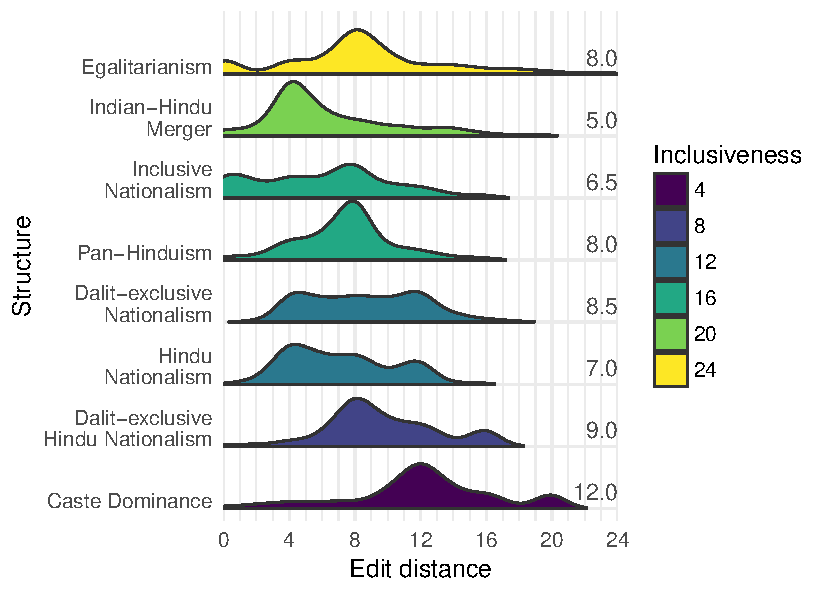
\includegraphics[scale=1]{../figures/appendices/appendices-b-1}
\caption[Edit distances between social identity structures and participants' responses]{Edit distances between each social identity structure and participants' responses. Edit distance is the sum of all categorizations in which a participant's responses differed from the ones implied by the proposed structure. Numbers (on the right) show the median edit distance per structure. %Points indicate the median \emph{social identity inclusiveness} of participants' responses at a specific edit distance.
}
\label{fig:b-1}
\end{figure}

Overall, participants' responses most closely resembled the Indian-Hindu merger structure ($\textit{Mdn} = 5.0$), in which participants include all targets who are \emph{either} Indian \emph{or} Hindu \emph{or} both in the ingroup. This was closely followed by inclusive nationalism ($\textit{Mdn} = 6.5$), i.e. participants include all targets who are Indian, and Hindu nationalism ($\textit{Mdn} = 7.0$), i.e. participants include only Indian Hindu targets. In addition, Pan-Hinduism ($\textit{Mdn} = 8.0$), i.e. participants include all Hindu targets, and egalitarianism ($\textit{Mdn} = 8.0$), i.e. participants include all targets, somewhat described participants' responses. Caste did not seem to dominate participants' responses ($\textit{Mdn} = 12.0$). Together, these observations suggested that, on the broadest level of analysis, participants relied on nationality and religion, rather than caste, to define their ingroup.

\section{Appendix C: Intergroup Threat}

We tested whether participants' perceptions of \emph{realistic} and \emph{symbolic threat} differed depending on the inclusiveness of their ingroup construals. Specifically, we examined whether participants reported feeling less threatened by Muslims and Dalits if they categorized more targets from these outgroups as ``us'' versus ``not us''. We excluded responses from Scheduled Caste/Scheduled Tribe participants to Scheduled Caste/Scheduled Tribe targets as we were interested in perceptions of \emph{inter}group threat. Models~0 to 7 estimated participants' mean responses, between $1 = \textit{strongly disagree}$ and $5 = \textit{strongly agree}$, to each of the $ 5 (\text{items}) \times 2 (\text{outgroups}) = 10$ items. Models derived the likelihood of the observed responses from the normal likelihood distribution: $$ y_{ij} \sim \text{Normal} (\mu_{ij}, \sigma) $$ where $y$ is the vector of participants' responses to each item, and $\mu_{ij}$ is the estimated mean response to item $i$ by participant $j$, $\sigma$ is the estimated residual variance (expressed as standard deviation).

Models~0 to 3 tested whether participants' responses differed across the two subscales (realistic vs symbolic threat) and across the two outgroups (Muslims vs Dalits).  Model 0 estimated item responses as varying between participants but fixed across all items: $$ \mu_{ij} = \beta_0 + \beta_{j} $$ where $\mu_{ij}$, the estimated mean response to item $i$ by participant $j$, equals $\beta_0$, the fixed intercept across items and participants, plus $\beta_j$, the varying intercept for participant $j$. Instead of assigning the same mean to all items, Model~1 included distinct intercepts for the two subscales: $$ \mu_{ij} = \beta_k + \beta_{j} $$ where $\beta_k$ is the fixed intercept for all items $i$ in subscale $k$, with $k = 1$ for realistic threat and $k = 2$ for symbolic threat. Model 2 instead estimated distinct intercepts for items concerning the two outgroups: $$ \mu_{ij} = \beta_l + \beta_{j} $$ where $\beta_l$ is the fixed intercept for all items $i$ for outgroup $l$, with $l = 1$ for Dalits and $l = 2$ for Muslims as the relevant outgroup. Model 3 tested the interaction of the two factors, and estimated distinct intercepts for all four combinations of subscales and outgroups: $$ \mu_{ij} = \beta_m + \beta_{j} $$ where $\beta_m$ is the fixed intercept for realistic threat from Dalits (when $m = 1$), for symbolic threat from Dalits (when $m = 2$), for realistic threat from Muslims (when $m = 3$), and for symbolic threat from Muslims (when $m = 4$). 

\begin{table}
\centering
\figureversion{lining, tabular}
\caption[Model comparison for intergroup threat]{Comparison of models estimating participants' intergroup threat. We preferred a more complex model over a simpler model when $\frac{\Delta\textit{ELPD}}{\textit{SE}} \geq 2$.}
\small	
\begin{tabularx}{\linewidth}{r@{~}rXrrrrrrr} \toprule
\# &  &  Description &  $R^2$ & $\textit{ELPD}$ & $\textit{SE}$ & $\Delta\textit{ELPD}$ & $\textit{SE}$ & $\frac{\Delta\textit{ELPD}}{\textit{SE}}$ & $w$ \\ \midrule \addlinespace
0 &      & \textit{Varying intercept} & .31 & -3368.1 & 32.9 & - & - & - & .11 \\
1 & vs 0 & \textit{Subscales}         & .31 & -3368.9 & 32.9 & -0.8 & 0.6 & -1.3 & .00 \\
2 & vs 0 & \textit{Outgroups} & .32 & -3363.7 & 33.0 & 4.4 & 3.3 & 1.3 & .00 \\
3 & vs 0 & \textit{Subscales $\times$ Outgroups} & .33 & -3335.1 & 34.0 & 33.0 & 8.4 & 3.9 & .19 \\ \midrule
4 & vs 3 & \textit{Categorizations}   & .33 & -3335.5 & 34.0 & -0.3 & 0.6 & -0.5 & .00 \\
5 & vs 3 & \textit{Categorizations}   & .34 & -3330.5 & 34.0 & 4.7 & 3.6 & 1.3 & .71 \\
6 & vs 3 & \textit{Categorizations}   & .33 & -3336.7 & 34.0 & -1.5 & 0.7 & -2.1 & .00 \\
7 & vs 3 & \textit{Categorizations}   & .34 & -3332.8 & 34.0 & 2.3 & 3.6 & 0.6 & .00 \\ \addlinespace \bottomrule
\end{tabularx}
\label{tab:c-1}
\end{table}

Model~3, but not Models 1 and 2, improved upon the predictions of Model~0 (Table~\ref{tab:c-1}), showing that participants' perceptions of symbolic and realistic threat depended on whether the relevant outgroup was Muslims or Dalits. Specifically, participants reported more realistic ($ \beta_1 = 3.62$, $[3.49, 3.75]$) than symbolic ($\beta_2 = 3.21$, $[3.09, 3.33]$) threat from (same-religion) Dalits, $\text{Pr} (\beta_1 > \beta_2|M3) > .99$, but less realistic ($\beta_3 = 3.23$, $[3.06, 3.38]$) than symbolic ($\beta_4 = 3.47$, $[3.34, 3.61]$) threat from (different-religion) Muslims, $\text{Pr} (\beta_3 < \beta_4| M3) > .99$.

Models 4 to 7 tested whether the proportion of \emph{Indian, Muslim, OBC} and \emph{Indian, Hindu, SC/ST} targets participants had categorized as ``us'' was associated with less perceived threat from, respectively, Muslims and Dalits. Model~4 estimated this relationship as constant across outgroups and subscales: $$ \mu_{ij} = \beta_m + \beta_{j} + \beta_{Q1}x_{Q1,jl} $$ where $x_{Q1,jl}$ is the proportion [0--1] of targets belonging to outgroup $l$ that participant $j$ categorized as ``us'', and $\beta_{Q1}$ estimates the difference in threat perceptions between participants who categorized all four targets of outgroup $l$ as ``us'' and participants who categorized all targets of outgroup $l$ as ``not us''. Models~5 to 7 instead estimated distinct coefficients $\beta_{Q1,k}$ for each of the two subscales (M5), $\beta_{Q1,l}$ for each of the two outgroups (M6), or $\beta_{Q1,m}$ for each of the four combinations of subscales and outgroups (M7). Other than expected, Models~4 to 7 did not make better out-of-sample predictions than Model 3, indicating that whom participants considered ``us'' and ``not us'' was not associated with their perceptions of intergroup threat.

\section{Appendix D: Support for Social Change}

We used the following analytic strategy: First, we tested for \emph{group differences} in participants' perceptions of (dis-)advantage and in their support for affirmative action. Second, we analysed to what extent contact experiences and ingroup construals explained \emph{individual differences} in participants' responses. We examined participants' responses to measures concerning outgroup members to test the \emph{solidarity hypothesis} (that positive contact encourages advantaged-group members to support social change). We examined participants' responses to measures concerning their ingroup to test the \emph{demobilisation hypothesis} (that positive contact discourages disadvantaged-group members from supporting social change) and the \emph{mobilisation hypothesis} (that negative contact encourages disadvantaged-group members to support social change).

\subsubsection{Group differences}

We investigated how participants' caste memberships shaped their perceptions of life difficulty and their support for reservations. To that end, we estimated two Bayesian multivariate models in \emph{RStan} \cite{rstan_package} with participants' responses to six perceived life difficulty and three policy support measures as outcome variables.\footnote{For this analysis, we aggregated items so that target groups corresponded across the two outcome measures. For perceived life difficulty, we aggregated items for Scheduled Caste and Scheduled Tribe groups, resulting in six variables. For policy support, We aggregated items for Scheduled Castes / Scheduled Tribes reservations, and for Other Backward Classes reservations, resulting in three variables.} Both models estimated how participant $j$ responded to each of the nine outcomes. Models derived the likelihood of the observed responses from a multivariate normal distribution: $$ \textbf{Y} \sim \text{MVNormal} (\mu_{jk}, \textbf{S} ) $$ where $\textbf{Y}$ is the matrix of observed variable scores (columns) across participants (rows), $\mu_{jk}$ is the estimated response to item $k$ by participant $j$, and $\textbf{S}$ is the variance-covariance matrix across variables. This means that models estimated distinct means and residual variances for each outcome, as well as residual correlations between all outcomes. Models assigned weakly informative priors to all intercepts, coefficients, and residual variances: 
\begin{align*} 
\beta & \sim \text{Normal} (0, 1) \\ 
\sigma & \sim \text{Cauchy} (0, 1)
\end{align*}
allowing a wide range of plausible effect sizes. Model~0 estimated distinct means for each outcome, but did not consider participants' group memberships: $ \mu_{jk} =  \beta_k $, where $\mu_{jk}$ equals $\beta_{k}$, the fixed intercept for outcome $k$. Model~1 estimated distinct means across participants' ingroups: $ \mu_{jk} =  \beta_k + \beta_{k,\text{OBC}} + \beta_{k,\text{SCST}} $, where $\mu_{jk}$ equals $\beta_k$, the fixed intercept for outcome $k$, plus $\beta_{k,\text{OBC}}$ and $\beta_{k,\text{SCST}}$, the coefficients estimating by how much Other Backward Class and Scheduled Caste~/ Scheduled Tribe participants' responses differed from General Merit participants'. Model~1 made better out-of-sample predictions than Model~0, $\Delta\textit{ELPD} = 94.7$, $SE = 14.1$, $\frac{\Delta\textit{ELPD}}{\textit{SE}} = 6.7$. This comparison shows that participants' caste memberships shaped their perceived discrimination and policy support ratings. 

Figure \ref{fig:ch5-s4-1} shows estimated mean ratings of perceived life difficulty for all target groups as a function of participants' caste memberships in Model~1. For most target groups, General Merit and Other Backward Class participants' responses closely resembled each other. On average, General Merit~/ Other Backward Class participants thought that it was somewhat hard (below the midpoint) for ``people from [their] own background'' to succeed. General Merit~/ Other Backward Class participants agreed with each other that it was a lot easier for people from Scheduled Caste~/ Scheduled Tribe backgrounds to succeed, compared to people from their own background. General Merit~/ Other Backward Class participants also agreed that, of all target groups, life was most difficult for people from General Merit backgrounds. Other Backward Class participants disagreed with General Merit participants when rating life difficulty for people from Other Backward Class backgrounds. General Merit participants rated life difficulty for Other Backward Class people as somewhat easy, while Other Backward Class participants tended toward ``neither easy nor hard'' and ``somewhat hard''. Scheduled Caste~/ Scheduled Tribe participants' responses differed markedly from General Merit and Other Backward Class participants'. For all target groups, Scheduled Caste~/ Scheduled Tribe participants rated life difficulty as ``neither easy nor hard'', on average. General Merit, Other Backward Class, and Scheduled Caste~/ Scheduled Tribe participants all tended to rate life difficulty for Muslims as around the midpoint. Overall, participants' responses seemed to contradict, or even reverse, persisting social inequalities (see Chapter~4, \emph{Caste, religion, and nation in South India}).

\begin{figure}
\centering
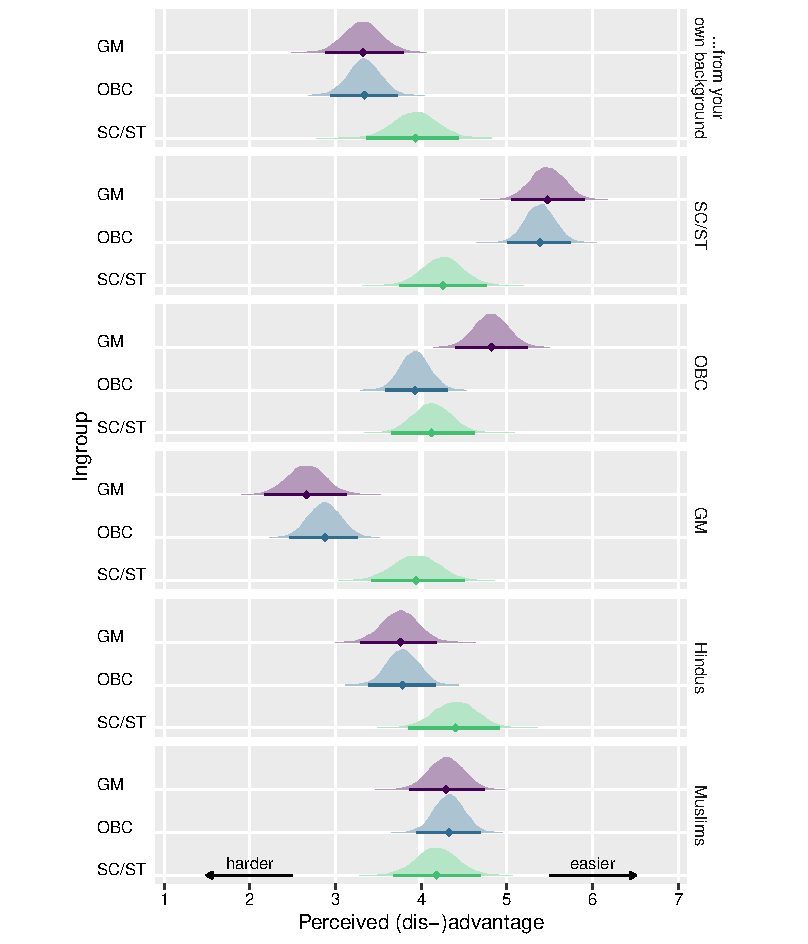
\includegraphics[scale=1]{../figures/figure-7}
\caption{
Posterior probabilities of perceived (dis-)advantage ratings for different target groups (right) by participants' caste ingroup (left). Diamonds mark the most plausible estimate of each mean rating; intervals encompass the 97\% most plausible estimates. GM = General Merit, OBC = Other Backward Class, SC/ST = Scheduled Caste/Scheduled Tribe.
}
\label{fig:ch5-s4-1}
\end{figure}

Figure \ref{fig:ch5-s4-2} shows estimated policy support---that is, support for reservations benefiting Scheduled Caste~/ Scheduled Tribe, Other Backward Class, and Muslim students---as a function of participants' caste memberships in Model~1. General Merit and Other Backward Class participants' responses did not provide evidence for cross-group solidarity. General Merit participants tended to oppose reservations for Scheduled Caste~/ Scheduled Tribe ($M = 1.87$, $[1.63, 2.12]$), Other Backward Class ($M = 2.70$, $[2.44, 2.96]$), and Muslim students ($M = 2.75$, $[2.46, 3.01]$). Other Backward Class participants tended to support reservations for their own group ($M = 3.72$, $[3.50, 3.95]$), but not for Scheduled Caste~/ Scheduled Tribe ($M = 2.31$, $[2.10, 2.53]$) or Muslim ($M = 2.79$, $[2.55, 3.04]$) students. Scheduled Caste~/ Scheduled Tribe participants tended to support reservations for their own group ($M = 4.16$, $[3.88, 4.45]$), for Other Backward Class students ($M = 3.57$, $[3.27, 3.86]$), and, to a lesser extent, for Muslim students ($M = 3.24$, $[2.92, 3.57]$). Overall, participants' responses provided evidence for solidarity from Scheduled Caste~/ Scheduled Tribe participants to Other Backward Class students, but not for solidarity from General Merit and Other Backward Class participants to Scheduled Caste~/ Scheduled Tribe students. 

\begin{figure}
\centering
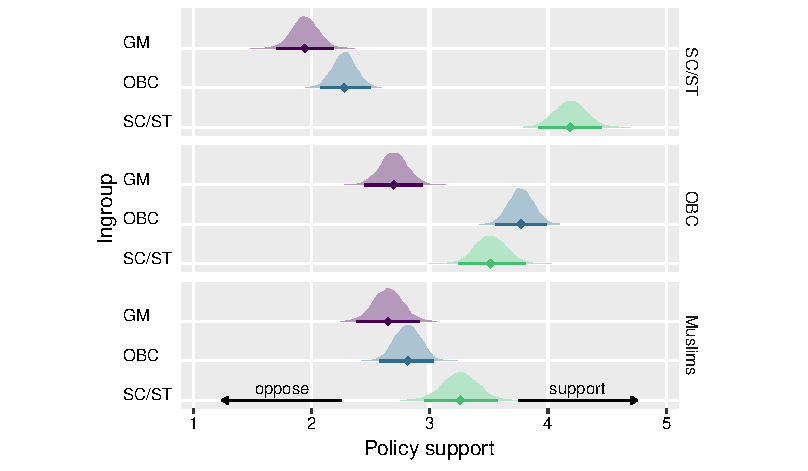
\includegraphics[scale=1]{../figures/figure-8}
\caption{
Posterior probabilities of policy support ratings for different target groups (right) by participants' caste ingroup (left). Diamonds mark the most plausible estimate of each mean rating; intervals encompass the 97\% most plausible estimates. GM = General Merit, OBC = Other Backward Class, SC/ST = Scheduled Caste/Scheduled Tribe.
}
\label{fig:ch5-s4-2}
\end{figure}

\begin{table}
\centering
\figureversion{lining, tabular}
\caption[Estimated residual correlations in Models 0 and 1 for Study 4]{Estimated residual correlations between six \emph{perceived life difficulty} (PD) ratings and three \emph{policy support} (PS) ratings in Model~0 (below the diagonal) and Model~1 (above the diagonal) for Study 4.}
\small	
\begin{tabularx}{\linewidth}{rl@{~}Xrrrrrr|rrr} \toprule
\# & \multicolumn{2}{l}{Variable} & 1 & 2 & 3 & 4 & 5 & 6 & 7 & 8 & 9 \\ \midrule \addlinespace
1 & PD, & \ldots own background & \textbf{}  & .14 & .30 & .45 & .43 & .05 & .28 & .12 & .14 \\
2 & PD, & SC/ST  & .10 & \textbf{} & .33 & -.13 & -.09 & .28 & -.12 & -.10 & -.05 \\
3 & PD, & OBC    & .28 & .33 & \textbf{} & .20 & .16 & .32 & .05 & -.17 & -.13  \\
4 & PD, & GM     & .47 & -.18 & .18 & \textbf{} & .61 & -.08 & .24 & .15 & .02 \\
5 & PD, & Hindu  & .44 & -.12 & .15 & .62 & \textbf{} & -.01 & .29 & .11 & .03  \\
6 & PD, & Muslim & .04 & .28 & .31 & -.10 & -.02 & \textbf{} & .02 & -.17 & -.15 \\ \midrule
7 & PS, & SC/ST  & .29 & -.24 & -.03 & .33 & .30 & -.03 & \textbf{} & .24 & .34 \\
8 & PS, & OBC    & .11 & -.13 & -.25 & .17 & .12 & -.16 & .28 & \textbf{} & .47 \\
9 & PS, & Muslim & .16 & -.09 & -.13 & .06 & .05 & -.16 & .36 & .45 & \textbf{}   \\ \addlinespace \bottomrule
\end{tabularx}
\label{tab:ch5-s4-1}
\end{table}

Table~\ref{tab:ch5-s4-1} shows the estimated residual correlations before (Model~0) and after (Model~1) accounting for group differences. Perceiving a group to be disadvantaged correlated weakly with more support for reservations benefiting Scheduled Caste~/ Scheduled Tribe ($r = -.12 $, $[-.24,.01]$), Other Backward Class ($r = -.17$, $[-.30,-.05]$), and Muslim ($r = -.15$, $[-.28,-.03]$) students in Model~1. Support for reservations for one target group correlated moderately with support for reservations for the other target groups, $.24 < r < .47$. These correlations provided evidence for systematic variation in policy support ratings across participants, even after accounting for group differences. In the next section, we examine to what extent contact experiences and ingroup construals explain this variation across individuals.

\subsubsection{Individual differences}

We examined to what extent contact experiences and ingroup construals (measured as participants' responses in the crossed-categorization task) accounted for individual differences in perceived life difficulty and policy support. To that end, we estimated a series of Bayesian multilevel models with either perceived life difficulty or policy support as outcome variable. Models derived the likelihood of the observed responses from a normal distribution: $$ y_{ij} \sim \text{Normal} (\mu_{ij}, \sigma) $$ where $y_{ij}$ is the observed response to item $i$ by participant $j$, and $\mu_{ij}$ is the estimated response to item $i$ by participant $j$, $\sigma$ is the estimated residual variance (expressed as standard deviation). We used the same weakly informative priors as for the multivariate models.

First, we estimated participants' responses to each of five perceived life difficulty items, with General Caste (GM), Scheduled Caste (SC), Scheduled Tribe (ST), Other Backward Class (OBC), and Muslims as target groups. Model~0 estimated item responses as varying across participants and target groups, and estimated differences across participants' ingroups: $$ \mu_{ij} = \beta_{j} + \beta_{kl} $$ where $\mu_{ij}$, the estimated mean response to item $i$ by participant $j$, equals $\beta_j$, the varying intercept for participant $j$, and $\beta_{kl}$, the varying intercept for target group~$k$ ($1 = \text{GM}$, $2 = \text{OBC}$, $3 = \text{SC/ST}$, $4 = \text{Muslims}$) and ingroup~$l$ ($1 = \text{GM}$, $2 = \text{OBC}$, $2 = \text{SC/ST}$). Model~0 thus resembled the multivariate model estimated above. 

Model~1 extended Model~0 by estimating to what extent outgroup friendship and negative contact with outgroup members were associated with perceptions of life difficulty for outgroups: $$ \mu_{ij} = \beta_{j} + \beta_{kl} + \beta_\text{OF}x_{\text{OG},k}x_\text{OF,jk} + \beta_\text{NC}x_{\text{OG},jk}x_\text{OF,jk}$$ where $x_{\text{OG},jk}$ codes whether target group $k$ is an outgroup [1] or ingroup [0] for participant $j$, $x_\text{OF,jk}$ and $x_\text{NC,jk}$ are, respectively, participant $j$'s outgroup friendship and negative contact with target group $k$, and $\beta_\text{OF}$ and $\beta_\text{NC}$ estimate the increase in participants' ratings for each additional standard deviation of reported contact. Model~2 estimated the effects of outgroup friendship and negative contact on outgroup ratings as varying across target outgroups: $$ \mu_{ij} = \beta_{j} + \beta_{kl} + \beta_{\text{OF},k}x_{\text{OG},k}x_\text{OF,jk} + \beta_{\text{NC},k}x_{\text{OG},jk}x_\text{OF,jk}$$ where $\beta_{\text{OF},k}$ and $\beta_{\text{NC},k}$ estimate effects of contact on ratings for outgroup $k$. Neither Model~1 nor Model~2 improved upon the out-of-sample predictions of Model~0, showing that intergroup contact neither increased nor decreased participants' perceptions of discrimination against ethnoreligious or caste outgroups (see Table~\ref{tab:ch5-s4-2}).

Models~3 and 4 tested whether participants' ingroup construals were associated with their perceptions of life difficulty for various outgroups. Model~3 estimated this relationship as constant across target groups: $$ \mu_{ij} = \beta_{j} + \beta_{kl} + \beta_\text{Q1}x_{\text{OG},k}x_\text{Q1,jk} $$ where $x_{Q1,jk}$ is the proportion [0--1] of targets belonging to outgroup $k$ that participant $j$ categorized as ``us'', and $\beta_{Q1}$ estimates the difference in perceived life difficulty between participants who categorized all four targets of an outgroup as ``us'' and participants who categorized all targets of an outgroup as ``not us''. Model~4 estimated this relationship as varying across outgroups: $$ \mu_{ij} = \beta_{j} + \beta_{kl} + \beta_\text{Q1,k}x_{\text{OG},k}x_\text{Q1,jk} $$ where $\beta_{Q1,k}$ estimates the difference in perceived perceived life difficulty between participants who categorized all four targets of outgroup $k$ as ``us'' and participants who categorized all targets of outgroup $k$ as ``not us''. Neither Model~3 nor Model~4 improved upon the out-of-sample predictions of Model~0, showing that more inclusive identities neither increased nor decreased participants' perceptions of life difficulty for ethnoreligious an caste outgroups. % Overall, Models~1 to 4 did not provide evidence for the solidarity hypothesis or, more specifically, for the solidarity-by-inclusion hypothesis.

Models~5 to 8 tested to what extent contact with (Models~5, 6) and inclusion of advantaged-group members (Models~7, 8) was associated with perceptions of life difficulty for the ingroup. Model~5 estimated how contact with General Merit people affected Scheduled Caste~/ Scheduled Tribe participants' perceptions of life difficulty for their ingroup: $$ \mu_{ij} = \beta_{j} + \beta_{kl} + \beta_\text{OF,GM}x_{\text{IG,jk}}x_{\text{SCST,j}}x_\text{OF,GM,j} + \beta_\text{NC,GM}x_{\text{IG,jk}}x_{\text{SCST,j}}x_\text{NC,GM,j} $$ where $x_{\text{IG},jk}$ codes whether target group $k$ is an ingroup [1] or outgroup [0] for participant $j$, $x_{\text{SCST,j}}$ codes whether participant $j$ is from an Scheduled Caste~/ Scheduled Tribe background [1] or not [0], $x_\text{OF,j,GM}$ and $x_\text{NC,j,GM}$ are, respectively, participant $j$'s outgroup friendship and negative contact with General Merit people, and $\beta_\text{OF,GM}$ and $\beta_\text{NC,GM}$ estimate the increase in participants' ratings for each additional standard deviation of reported contact with General Merit people. Model~6 extended Model~5 by estimating how contact with General Merit people affected Other Backward Class participants' perceptions of life difficulty for their ingroup: $$ \mu_{ij} = \beta_{j} + \beta_{kl} + \ldots + \beta_\text{OF,GM}x_{\text{IG,jk}}x_{\text{OBC,j}}x_\text{OF,GM,j} + \beta_\text{NC,GM}x_{\text{IG,jk}}x_{\text{OBC,j}}x_\text{NC,GM,j} $$ where $x_{\text{OBC,j}}$ codes whether participant $j$ is from an Other Backward Class background [1] or not [0]. Neither Model~5 nor Model~6 improved upon the out-of-sample predictions of Model~0, showing that intergroup contact with advantaged-group members did not increase or decrease disadvantaged-group members' perceptions of life difficulty for their ingroup. Model~7 estimated whether including General Merit targets in their ingroup reduced perceptions of life difficulty among Scheduled Caste~/ Scheduled Tribe participants: $$ \mu_{ij} = \beta_{j} + \beta_{kl} + \beta_\text{Q1,GM}x_{\text{IG,jk}}x_{\text{SCST,j}}x_\text{Q1,GM,j} $$ where $x_{Q1,GM,j}$ is the proportion [0--1] of General Merit targets that participant $j$ categorized as ``us'', and $\beta_{Q1,GM}$ estimates the difference in perceived life difficulty between participants who categorized all four General Merit targets as ``us'' and participants who categorized all General Merit targets as ``not us''. Model~8 extended Model~7 by estimating this relationship among Other Backward Class participants: $$ \mu_{ij} = \beta_{j} + \beta_{kl} + \beta_\text{Q1,GM}x_{\text{IG,jk}}x_{\text{SCST,j}}x_\text{Q1,GM,j} + \beta_\text{Q1,GM}x_{\text{IG,jk}}x_{\text{OBC,j}}x_\text{Q1,GM,j} $$ where $x_{\text{OBC,j}}$ codes whether participant $j$ is from an Other Backward Class background [1] or not [0]. Neither Model~7 nor Model~8 improved upon Model~0, showing that including advantaged-group members in the ingroup did not increase or decrease disadvantaged-group members' perceptions of their ingroup's life difficulty (see Table~\ref{tab:ch5-s4-2}).

\begin{table}
\centering
\figureversion{lining, tabular}
\caption{
Comparison of models estimating participants' group-wise perceived life difficulty ratings. We preferred a more complex model over a simpler model when $\frac{\Delta\textit{ELPD}}{\textit{SE}} \geq 2$.
}
\small	
\begin{tabularx}{\linewidth}{r@{~}rXrrrrrrr} \toprule
\# &  &  Description & $R^2$ & $\textit{ELPD}$ & $\textit{SE}$ & $\Delta\textit{ELPD}$ & $\textit{SE}$ & $\frac{\Delta\textit{ELPD}}{\textit{SE}}$ & $w$ \\ \midrule \addlinespace
0 &      & \textit{Group differences} & .35 & -1789.5 & 24.6 & - & - & - & .00 \\ \addlinespace
1 & vs 0 & \textit{Solidarity}       & .35 & -1791.2 & 24.5 & -1.8 & 1.5 & -1.2 & .00 \\
2 & vs 1 & \textit{Solidarity}       & .35 & -1788.3 & 24.4 & 3.0 & 2.5 & 1.2 & .33 \\
3 & vs 0 & \textit{Solidarity}       & .35 & -1787.0 & 24.7 & 2.5 & 2.4 & 1.0 & .32 \\
4 & vs 3 & \textit{Solidarity}       & .35 & -1787.6 & 24.7 & -0.7 & 2.4 & -0.3 & .23 \\ \addlinespace
5 & vs 0 & \textit{(De)mobilisation} & .35 & -1791.5 & 24.6 & -2.0 & 1.2 & -1.7 & .00 \\
6 & vs 5 & \textit{(De)mobilisation} & .35 & -1792.6 & 24.6 & -1.1 & 0.9 & -1.2 & .00 \\
7 & vs 0 & \textit{(De)mobilisation} & .35 & -1788.9 & 24.5 & 0.5 & 1.4 & 0.4 & .00 \\
8 & vs 7 & \textit{(De)mobilisation} & .35 & -1788.4 & 24.5 & 0.5 & 1.4 & 0.4 & .12 \\ \addlinespace \bottomrule
\end{tabularx}
\label{tab:ch5-s4-2}
\end{table}

\begin{table}
\centering
\figureversion{lining, tabular}
\caption[Model comparison for individual differences in policy support for Study 4]{Comparison of models estimating participants' group-wise policy support ratings. As in Table~\ref{tab:ch5-s4-2}, we preferred a more complex model over a simpler model when $\frac{\Delta\textit{ELPD}}{\textit{SE}} \geq 2$.}
\small	
\begin{tabularx}{\linewidth}{r@{~}rXrrrrrrr} \toprule
\# &  &  Description & $R^2$ & $\textit{ELPD}$ & $\textit{SE}$ & $\Delta\textit{ELPD}$ & $\textit{SE}$ & $\frac{\Delta\textit{ELPD}}{\textit{SE}}$ & $w$ \\ \midrule \addlinespace
0 &      & \textit{Group differences} & .49 & -1741.0 & 26.8 & - & - & - & .00 \\ \addlinespace
1 & vs 0 & \textit{Solidarity}       & .50 & -1736.1 & 26.7 &  4.9 & 2.7 & 1.8 & .60 \\
2 & vs 1 & \textit{Solidarity}       & .50 & -1739.9 & 26.8 &   -3.8 & 2.0 & -1.9 & .00 \\
3 & vs 0 & \textit{Solidarity}       & .49 & -1741.0 & 26.9 & 0.0 & 0.7 & 0.0 & .00 \\
4 & vs 3 & \textit{Solidarity}       & .49 & -1741.6 & 26.9 &  -0.6 & 1.1 & -0.5 & .00 \\ \addlinespace
5 & vs 0 & \textit{(De)mobilisation} & .49 & -1742.0 & 26.9 & -0.9 & 1.7 & -0.5 & .03 \\
6 & vs 5 & \textit{(De)mobilisation} & .49 & -1743.3 & 26.9 & -1.3 & 0.8 & -1.6 & .00\\
7 & vs 0 & \textit{(De)mobilisation} & .49 & -1741.6 & 26.8 & -0.6 & 0.8 & -0.8 & .00\\
8 & vs 7 & \textit{(De)mobilisation} & .50 & -1740.0 & 26.8 &  1.6 & 2.0 & 0.8 & .37 \\ \addlinespace \bottomrule
\end{tabularx}
\label{tab:ch5-s4-3}
\end{table}

Second, we estimated participants' responses to each of five policy support items, with Scheduled Caste and Scheduled Tribe (SC/ST), Other Backward Class (OBC), and Muslims as target groups. Model~0 estimated item responses as varying across participants and target groups, and estimated differences across participants' ingroups: $$ \mu_{ij} = \beta_{j} + \beta_{kl} $$ where $\mu_{ij}$, the estimated mean response to item $i$ by participant $j$, equals $\beta_j$, the varying intercept for participant $j$, plus $\beta_{kl}$, the varying intercept for target group~$k$ ($1 = \text{SC/ST}$, $2 = \text{OBC}$, $3 = \text{Muslims}$) and ingroup~$l$ ($1 = \text{GM}$, $2 = \text{OBC}$, $2 = \text{SC/ST}$). Model~0 thus resembled the multivariate model estimated in the previous section. Models~1 to 8 were identical to the models for perceived discrimination (described above). Models~1 to 4 did not improve upon the out-of-sample predictions of Model~0, showing that neither intergroup contact (Models~1, 2) nor inclusive identities (Models~3, 4) foster support for policies benefiting a disadvantaged outgroup.  Models~5 to 8 did not improve upon the out-of-sample predictions of Model~0, showing that neither contact with (Models~5, 6) nor inclusion of (Models~7, 8) General Merit people affected Scheduled Caste~/ Scheduled Tribe and Other Backward Class participants' support for policies benefiting their ingroups (see Table~\ref{tab:ch5-s4-3}).

Overall, these findings show that neither intergroup contact nor ingroup construals could explain individual differences in support for social change. Contrary to the \emph{demobilisation hypothesis}, positive contact did not decrease disadvantaged-group participants' support for social change. Contrary to the \emph{mobilisation hypothesis}, negative contact did not increase disadvantaged-group participants' support for social change. Contrary to predictions, neither positive contact nor more inclusive identities were associated with support for policies benefiting (other) disadvantaged outgroups.

\section{Appendix E: Additional Measures}

\subsection{Measures}

Group identification was measured with one item per ingroup \cite{postmes_single_2013}: ``I identify with my [nationality/religion/caste group]'' ($1 = \textit{strongly disagree}$, $7 = \textit{strongly agree}$).

Social identity complexity \cite{roccas_social_2002, schmid_antecedents_2009} was operationalised as the extent to which participants perceived their different group memberships as conceptually interrelated (\emph{similarity complexity}) and numerically overlapping (\emph{overlap complexity}). Two items measured similarity complexity for religion/nationality and for nationality/caste: ``How similar or different are the typical [Hindu/Indian] and the typical [Indian/person from your caste group] to each other?'' ($1 = \textit{very different}$, $5 = \textit{very similar}$, reverse coded), and ``Do you think that being [Hindu/Indian] means the same as being [Indian/from your caste group]?'' ($1 = \textit{means something very similar}$, $5 = \textit{means something very different}$).  Two items measured overlap complexity for religion/nationality: ``How many [Indians/ Hindus] do you think are [Hindus/Indian]?” (\%, $r = .63$). Three items measured overlap complexity for nationality and caste: ``How many Indians do you think are [GC, OBC, SC/ST]?'' (\%, $.33 \leq rs \leq .50$). Overlap items were reverse coded, so that higher scores indicated less perceived overlap.

\emph{Entitativity} \cite{lickel_varieties_2000} was measured with six items: ``Being Indian is important to each Indian, no matter their caste or religion'', ``Indians of all castes and religions interact often with each other.'', ``Indians of all castes and religions are working towards shared goals'', ``What happens to one Indian also impacts other Indians'', ``Indians of all castes and religions depend on one another'', and ``Indians are similar to one another'' ($1 = \textit{strongly disagree}$, $7 = \textit{strongly agree}$, $\alpha = .80$). Participants were encouraged to ``take Indian/Indians to mean Indian citizens of all castes and religions'' when reading the items of this scale. This scale thus measured an inclusive conception of entitativity.

\subsection{Correlates of categorisation}

Aside from testing potential antecedents and consequences, I explored how participants' responses in the crossed-categorisation task related to other measures of social identification. To that end, I estimated the correlations between, on the one hand, the proportions of targets that participants had categorised as ``us'' in each of the six categories, and, on the other hand, the (aggregated) social identification variables described in the \emph{Measures} section. I derived the likelihood of the observed responses from a multivariate normal distribution: $$ \textbf{Y} \sim \text{MVNormal} (\mu , \textbf{S} ) $$ where $\textbf{Y}$ is the matrix of observed variable scores (columns) across participants (rows), $\mu$ is the vector of all variable means, and $\textbf{S}$ is the variance-covariance matrix across variables.

Figure~\ref{fig:ch4-appendix-1} shows the estimated correlations between participants' categorisations in the crossed-categorisation task (from left to right) and various social identification variables (from top to bottom). Entitativity---the extent to which participants saw Indians of \emph{all} castes and religions as similar to one another, as depending on each other, as sharing a common fate, as working towards shared goals, and as valuing their shared identity---was positively correlated with the proportion of \emph{Indian, Hindu, GM} ($r = .16$, $[.04, .27]$, $\text{Pr} (r > 0|M) > .99$), \emph{Indian, Hindu, OBC} ($r = .21$, $[.09, .31]$, $\text{Pr} (r > 0| M) > .99$), \emph{Indian, Hindu, SC/ST} ($r = .10$, $[-.02, .22]$, $\text{Pr} (r > 0| M) = .97$), and \emph{Indian, Muslim, OBC} ($r = .18$, $[.07, .30]$, $\text{Pr} (r > 0| M) > .99$) targets participants categorised as ``us''.

\begin{figure}
\centering
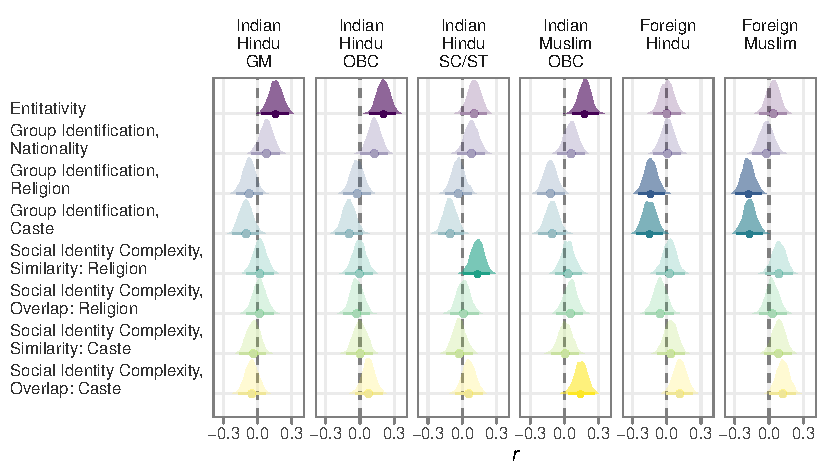
\includegraphics[scale=1]{../figures/appendices/appendices-e-1}
\caption[Correlations between social identity variables and target categorisations]{Correlations between various social identity variables (top to bottom) and the proportion of targets that participants had categorised as ``us'' in each target category (left to right). Points indicate the most likely estimate for a given correlation, while lines encompass the 97\% most likely estimates of that correlation. Curves show the density distributions of the posterior probabilities, based on all samples from the posterior probability distribution. Correlations for which $\text{Pr} (r > 0| M) > .99$ or $\text{Pr} (r < 0| M) > .99$ are shown in a darker shade.}
\label{fig:ch4-appendix-1}
\end{figure}

Group identification was only associated with participants' categorisations of foreign targets, not their categorisations of Indian targets. The extent to which participants identified with their religion was negatively correlated with how many \emph{foreign, Hindu} ($r = -.14$, $[-.25, -.02]$, $\text{Pr} (r > 0| M) > .99$) and \emph{foreign, Muslim} ($r = -.18$, $[-.29, -.07]$, $\text{Pr} (r > 0| M) > .99$) targets participant categorised as ``us''. I obtained similar correlations for the extent to which participants identified with their caste group, $r = -.15$, $[-.27, -.04]$, $\text{Pr} (r > 0| M) > .99$ and $r = -.17$, $[-.29, -.06]$, $\text{Pr} (r > 0| M) > .99$, respectively. The extent to which participants identified with their nationality was not associated with participants' categorisations---perhaps because there was a little variation in participants responses, with 81\% of participants strongly agreeing with the statement. Other variables were not systematically correlated with participants' responses in the crossed-categorisation task (see Figure~\ref{fig:ch4-appendix-1}).

Correlations thus confirmed that participants' categorisations were more than a straight-forward reflection of the strength of their group identification, affirming the value of the crossed-categorisation task for studying identification in contexts with multiple, cross-cutting group memberships. Furthermore, participants' perceptions of entitativity across caste and religions were associated with more inclusive construals of national identity, providing tentative evidence for its potential for fostering more inclusive identities.

\bibliographystyle{apacite}
\bibliography{references}

\end{document}